\chapter{Distinction to existing services}

\section{Vault}

Vault is a rather new service developed by \textit{Hashicorp}.
It offers a model to store and retrieve secrets, secured by a
master key which is split into shares and distributed to authorized
participants. Vault describes its use cases in conjunction with
server administration and orchestration activities for several users.
This overlaps with the goal specification of this project, but this aims
to be a more
consumer grade product and it focuses on the secret sharing algorithm.
Every secret should be split and be treated
as sensitive as Vault treats its master key. While the master key
could be a single point of failure for Vault, secrets in the target implementation
should still be safe even if one secret is unveiled or a private key
is made public. Also, the target is a product which has a strong focus
on software craftsmanship: A high level implementation which
makes it easy for others to contribute and to write additional
software while Vault is written in rather low-level go code. This
code also meets various QA criteria, but will not be as understandable
as the code inside the desired technology stack.
\cite{vault}

\section{Lastpass}

The use case of Lastpass is the management of personal passwords.
It is possible to share passwords with other people, but Lastpass
uses public key crypto here instead of secret sharing. The goal of this
is to focus more on the implementation of secret sharing
and the ability to split a secret than Lastpass. The other distinction
here is that this should be a solution which is available open source and
which can be hosted by anyone and Lastpass is a closed source
solution.

\section{KeePassX}

KeePassX is rather an offline solution. There is a key database file
which contains all sensitive information. If one wants to unlock this,
one has to use his master password. Cross platform use with KeePassX is rather
difficult, because the key database file would have to be synced
across many devices. Also, if the master password is stolen, the whole
key database is public - in contrast, secrets should be safe if
one secret is unveiled using the planned system. That system should also
take care of the safe distribution of one's secrets.

\chapter{Cryptography Fundamentals}

\section{Definition}

In present and past it is and always has been important for messages to be
transmitted securely and without the danger of information disclosure. To meet
these requirements, two main techniques have emerged:

One technique is called steganography. This discipline focuses on hiding the
transmission of messages. An example for this can be found in the past: To hide
a message, one used to shave off all hairs of a messenger. Then, the message
was tattooed on the skin. After a while, when the hair grew back, the messenger
was sent to the receiver. Border controls didn't notice this kind of message
transmission at the beginning, but after a while, the controls were informed to
check if a person was transmitting that kind of message. It was genius to
covertly transmit a message, but as soon as the message was discovered, the
information was disclosed. As a result, the message itself should have some
protection, so that only the desired receiver could read it. This was the point
in time when cryptography was born.

Cryptography is the art of encrypting a message so that only receivers with
specific knowledge can obtain the plain text. The first steps in cryptography
were simple so called substitution ciphers, when some symbols in an alphabet
were switched or rotated.

Imagine the following message:

\vspace{0.5cm}
\textit{attack at dawn}
\vspace{0.5cm}

If one substituted all "a"s with a "z" and all "t"s with an "e", the message
would look like this:

\vspace{0.5cm}
\textit{zeezck ze dzwn}
\vspace{0.5cm}

The message immediately becomes unreadable for someone who doesn't know about
the underlying substitution. As a measure to break this, cryptanalysis comes in:
If one looks
at the text, one could for example analyze the frequency of some specific
letters, in this example "z" and "e". The most common letters in the English
alphabet are "e" and "a". One could now try to substitute the letter "z" with
"e". The outcome would be

\vspace{0.5cm}
\textit{aeeack ae dawn}
\vspace{0.5cm}

If one can't guess that the message is \textit{attack at dawn}, one could
continue using cryptanalysis. Since substituting "e" with commonly used letters
fails, one could analyze two letter chains. One of the most common used two
letter combinations with "a" is "at" (as one could have guessed when seeing
"ae").  After substituting "e" with "t", the original message is revealed.

\vspace{0.5cm}
\textit{attack at dawn}
\vspace{0.5cm}

Soon, this procedure also became quite insecure and cryptographers tried to
find new ways to encrypt their messages. It was a gift for them when computers
became commonly available: Procedures requiring masses of mathematical
operations could be executed in less than a second, more complex encryption
algorithms appeared.

In modern cryptography there are two main kinds of encrypting and decrypting a
message. The first kind (which was actually also the first one that emerged) is
called \textit{symmetric encryption}. This kind of cryptography uses the same
key for en- and decryption of a message. The previously mentioned substitution
cipher is a \textit{symmetric encryption}, where the substitution table is the
key which is used for en- and decryption.

The other encryption kind is called \textit{asymmetric encryption}. Here, en-
and decryption are seen as different operations. That's why one has to use an
encryption and a decryption key to perform \textit{asymmetric encryption}.
\cite{singh2000geheime}

\section{Cryptographic primitives}

The most basic building blocks in the field of cryptography are known as
cryptographic primitives. They include well researched, reliable and accepted
algorithms. Digital signatures, one-way hash functions and public key
cryptography are examples for cryptographic primitives.

\subsection{Random numbers}

Random numbers are one of the main building blocks of modern cryptography.
Inside RSA (see section \ref{sub_sec:rsa}) they are used to create many
different encryption results even if always the same secret is being encrypted.
But what if the random numbers are not ``random enough''?

\paragraph{True Randomness}
True randomness is difficult to achieve in cryptography. Human behaviour
is likely to be predicted. As such, humans are bad sources of true randomness.
If one wants to obtain true randomness, the probably best source are physical
random number generators. Physical random number generators use underlying
physical processes to obtain randomness. An example of such a physical process
is the atmospheric noise or radioactive sources. Both can be measured and
are used to create good random numbers.

\paragraph{Pseudorandom numbers}
True random numbers are unpredictable, but today many random numbers per
second are needed in order for some cryptographic protocols to work. It would
take too long to generate a random number using a source of true randomness
every time. Modern computers generate random numbers by using a predefined behaviour.
They do some computations based on some merely random data and try to output
random numbers. The fact that these numbers are not truly random explains the name.
They are called \textit{pseudorandom} numbers  and the algorithms which create
them \textit{pseudorandom number generators}. Some of the existing algorithms
are rather easy to predict and some of them are not. For many use cases like
genetic algorithms, predictable sources of randomness are satisfactory
good enough to use because they offer high speed access to many random numbers.
However for cryptographic reasons, these numbers are not suitable. If one is
able to predict random numbers in a cryptographic protocol, it is easier to
make conclusions regarding the encrypted secret (which could happen for example
in RSA). Therefore, pseudorandom numbers have to be \textit{cryptographically}
secure in order to be used for encryption. Such cryptographically secure pseudorandom
number generators or short \textit{CSPRNG} work the same as ordinary pseudorandom
number generators with the difference being that they have to produce number sequences
which are not predictable and with which it is not possible to guess the internal
state of the random number generators. CSPRNGs can rely on cryptographic primitives
or on number theoretic designs.

\subsubsection{Blum Blum Shub}

The Blum Blum Shub CSPRNG is a random number generator which is based on a number
theoretic design. It was developed by Lenore Blum, Manuel Blum and Michael Shub
(which is where the name originates from) in 1986. The Blum Blum Shub generator needs
two primes $q$ and $p$ to work. Both primes have to be of the form $4k + 3$. Also,
the starting number $s_0$ has to be coprime to the modulus $n$.
Once both $s_0$ and $n$ have been determined, the following random number $s_{i+1}$ is
calculated as follows:

$$s_{i+1} = s_{i}^2 \Mod n$$

In general, the security of the Blum Blum Shub CSPRNG is determined by the
difficulty of the factorization of the modulus $n$. Since it is very difficult
to factorize huge $n$, Blum Blum Shub is considered safe if one uses a large
modulus.

\cite{blum1986simple}

\subsection{Prime numbers}

Prime numbers are natural numbers which are greater than one and only evenly
divisible by one and themselves.

Those numbers play a main role in cryptography as they are commonly used
as a security factor. For example, it is quite difficult to determine the
prime factorization of a number, as none of the existing algorithms solves
the problem in polynomial time. Therefore, prime factorization is a problem
of \textit{nondeterministic polynomial time complexity} and to factorize
large numbers, more time than the age of the universe is needed.

But how can one get prime numbers in a short amount of time? There are two
main known solutions: The first solution is to permute through all positive
natural numbers, more efficient algorithms here are for example the
\textit{Sieve of Eratosthenes} or the \textit{Sieve of Atkin}. The other
main approach is the statistical or heuristic approach. Well known methods
here are the \textit{Miller Rabin Test}, a test which delivers the probability
of a number to be a prime or not. This test is used in \textit{OpenSSL} to
find large primes, which makes it possible for users of \textit{OpenSSL} to
not have primes as factors of their RSA modulus.

\subsection{Chinese remainder theorem}

Given $k$ positive integers $n_1, \ldots, n_k$ which are pairwise coprime\footnote{
  Pairwise coprimality is fulfilled if a set is \textit{set-wise coprime},
  which means that the greatest common divisor of all elements in the set
  is $1$ and also each pair in the set is coprime.
}. For any given sequence of $i$ integers  $a_1, \ldots a_i$, there is an integer
$x$ which is congruent\footnote{
  A number is congruent another number if they output the same remainder
  after a modulo operation with the same modulus.
}
with all $a$s with the integers $n$:

$$
\left\{
\begin{array}{l l l}
  x \equiv a_1 \Mod n_1 \\
  \ldots \\
  x \equiv a_k \Mod n_k
\end{array}
\right.
$$

Additionally all solutions $x$ are also congruent modulo the Product $N = n_1 \ldots n_k$.

\cite{ding1996chinese}

\subsection{RSA}
\label{sub_sec:rsa}
	
RSA is an asymmetric encryption standard, developed by Ronald L. Rivest, Adi Shamir and
Leonard Adleman. As many other asymmetric encryption algorithms, RSA uses a one way function
with a trapdoor. So in order to understand RSA, one has to understand the
trapdoor function. The RSA trapdoor function relies on Euler's totient function
$\phi$. This function returns the amount of numbers which are relatively prime
and smaller than a number n. Since prime numbers are only evenly divisible by
1 and themselves, the totient function returns $n - 1$ for prime numbers. Also,
if you multiply a number with another, the totient function also multiplies
with the totient function of the other number. An example:

$$\phi(13) = 12$$

$$\phi(11) = 10$$

$$13 * 11 = 143$$

$$\phi(143) = \phi(13) * \phi(11) = 120$$

RSA uses this as follows: To encrypt something, one needs the so called
public key. To decrypt something, one needs the private key. Both keys
contain the so called RSA modulus \textit{n}, which is the product of 
two primes, \textit{p} and \textit{q}. The public key additionally has
the number \textit{e} and the private key has the additional number
\textit{d}. \textit{e} is a number which is coprime to the result of
the totient function of \textit{n}. \textit{d} is the multiplicative inverse
\footnote{The multiplicative inverse of a number $a$ is the number $b$ where $a*b = 1$} of
\textit{e} relative to $\phi(n)$.

Having calculated those needed factors, it is easy to en- and decrypt
a message representative (usually a number). To encrypt a message, one
has to apply the following procedure:

$$c = m^e \Mod{N}$$

Where \textit{c} is the ciphertext and \textit{m} the message representative.

The decryption follows the same procedure, only \textit{c} and \textit{d} are
swapped and the exponent is \textit{d}:

$$m = c^d \Mod{N}$$

Using this procedure without further additions isn't considered safe today:
One plaintext would always produce the same ciphertext. This is why cryptographers
started to use \textit{paddings}. Paddings wrap the plaintext and the padded
text is then encrypted. After decryption, the padding has to be removed in order
to obtain the original plaintext. As a result, to en- and decrypt a message, one
has to know the RSA procedure as well as the used padding.

There are several known so called \textit{padding schemes}. The most widespread
padding was defined in \textit{PKCS \#1}\cite{jonsson2003public}, the first of a family of standards
called Public Key Cryptography Standards. To encrypt, a secret Integer $m$ is 
first encoded into an octet string using the $i2osp$ (integer to octet string 
primitive). This results in an octet string message $M$. $M$ is then
concatenated with a randomly generated octet string as well as some other control
sequences as follows:

$$EM = 0x00 || 0x02 || PS || 0x00 || M$$

Where $EM$ is the encoded message and $PS$ the randomly generated octet string.
$EM$ is then converted into the ciphertext representing integer $C$ with the $os2ip$
operation (octet string to integer primitive).

The decryption then decodes $C$ back into $EM$ and 
uses the leading $0x00$ and $0x02$ to check if the padding was
applied. If so, it uses the second $0x00$ to detect the start of the encrypted
message. In total, this encryption padding enables users to encrypt secrets with
always different integer outcomes.

\cite{rivest1978method}

\subsection{AES}

AES is the short form for \textit{Advanced Encryption Standard}. It is a block cipher
and the successor of \textit{DES}. It is also often referred as \textit{Rijndael}
because of John Daemen and Vincent Rimen, who created the name as a play on their
names. It was submitted by them to the American NIST (National Institute of
Standards and Technology) when NIST was publicly searching for a successor of
DES.

\subsection{Criteria for the algorithm}

Each secure symmetric cipher has two main properties:
\textit{confusion} and \textit{diffusion}. Confusion tries to obfuscate
the relation between ciphertext and the key. Diffusion wants to
destroy the structure of the original text in the resulting ciphertext.
Additional to these two criteria, AES should be fast in software implementations
as well as in hardware realizations and also be space efficient for use
inside, for example, smart cards. At the time of writing, AES fulfills these
criteria and is used for strictly confidential documents inside the American
secret services.

\subsubsection{Procedure}

The algorithm executes as follows \cite{wikipedia_aes}:
\begin{enumerate}
  \item Key expansion
  \item Preliminary round
    \begin{itemize}
      \item AddRoundKey(Keys[0])
    \end{itemize}
  \item Encryption rounds (r = 0 to R - 1)
    \begin{itemize}
      \item SubBytes
      \item ShiftRows
      \item MixColumns
      \item AddRoundKey(Keys[i]) 
    \end{itemize}
  \item Final round
    \begin{itemize}
      \item SubBytes
      \item ShiftRows
      \item AddRoundKey(Keys[R]) 
    \end{itemize}
\end{enumerate}

In the final round, the bytes don't need to be mixed because the resulting
mixture wouldn't affect the next round and is therefore useless.
Hereafter, the main parts \textit{key expansion}, \textit{SubBytes},
\textit{MixColumns} and \textit{AddRoundKey} are explained.

\paragraph{Key expansion}
The key expansion generates $R + 1$ keys out of the user predefined key.
$R$ is the number of encryption rounds which in turn dependends on the key 
bit size (supported sizes are 128, 192 and 256 bits). Also,
the keys are adjusted to fit the block size.

\paragraph{SubBytes}
SubBytes substitutes the bytes by putting them into substitution boxes (sbox).
This will map each byte to another and represents a monoalphabetic substitution
and fulfills the \textit{confusion} criteria.

\paragraph{ShiftRows}
The ShiftRows step applies a shifting operation to the input bytes. This step
fulfills the \textit{diffusion} criteria each good encryption algorithm should
contain.

\paragraph{AddRoundKey}
This step is rather simple: Each byte is XORed with the current round key.

\cite{daemen20018}

\section{Cryptographic Protocols}

A cryptographic protocol is a combination of cryptographic primitives,
algorithms and possibly other cryptographic protocols. The protocol describes
how the cryptographic algorithms are used in order to increase confidentiality,
integrity and availability of the underlying goal.

Cryptographic protocols are usually defined abstract in order to leave language
specific difficulties up to the implementation. Since only the interfaces are
defined, the developers can implement against those and therefore make sure
different implementations are compatible to each other.

\subsection{Diffie-Hellmann}

The Diffie-Hellmann key exchange is a protocol to create a secret key between
two stations. A simple visualization of the Diffie-Hellmann key exchange can
be achieved by using colors. Imagine each of two persons has got a color,
their secret color. To now create a shared secret, they both agree on a
public color. After that, they mix their own private color with that public
color and send the mixture to each other. Both persons are now able to mix
the received mixture with their private color and have then both the same
color, their shared secret.

The previous description is rather informal. To turn those mentioned components
into a procedure which works with computers, some math is required.

First, there has to be a problem, which can't be solved in feasible time
(most commonly, it is an $NP$ hard problem). The most common problem for
the Diffie-Hellmann key exchange is the so called
\textit{Computational-Diffie-Hellmann Problem}:

\vspace{1em}

Given $g$ of a group and the values $A = g^a$ and $B = g^b$, what is
$K = g^{ab}$ with $a$ and $b$ unknown?

\vspace{1em}

The group $g$ is in today's use cases a \textit{cyclic group of prime order}.
In such groups, results of addition and multiplication are repeating
themselves. This is achieved by applying the modulo operation to the result
of e.g. an addition. The modulus has to be a prime number here. An example
for such a group would be

$$n \Mod{13}$$ where $13$ is the prime number and $n$ can be any number.

In practice, the commonly shared secret in the Diffie-Hellman key exchange
is the prime number $p$ determining the cyclic group of prime order and also
the number $g$ which is the base for that group ($g$ has to be a primitive
root of $p$, but explaining this is not relevant for the further explanation).
For the following example, $p = 23$ and $g = 5$.

After having shared the prime number, both participants generate their
private numbers $a$ and $b$, for example $a = 4$ and $b = 10$. Referring to the
previously mentioned visualization, $a$ and $b$ are the private colors of the
two persons wanting to communicate. They both then compute the mixture of their
private color and the ``color'' $g$ with $A = g^a$ and $B = g^b$ which is
$A = 5^4 \Mod{13} = 625 \Mod{13} = 1$ and $B = 5^{10} \Mod{13} = 9765625 \Mod{13} = 12$.

The mixtures are then transferred to the communication partner. Each
participant then computes the shared secret $s$ by raising the mixture
to the power of their private color. This results in the following:

$$s = B^a \Mod{p} = 12^4 \Mod{13} = 20736 \Mod{13} = 1$$

or

$$s = A^b \Mod{p} = 1^10 \Mod{13} = 1 \Mod{13} = 1$$

All in all, the Diffie-Hellmann key exchange provides a very secure way
to create a shared secret, but it is not bulletproof. It is vulnerable
to man-in-the-middle attacks:

Imagine Alice and Bob want to establish a shared secret. They proceed as
described previously by choosing their private colors and the numbers $g$
and $p$. But when asking each other for the mixture, the man in the middle
intercepts as follows: He blocks the request and instead returns a mixture
with his private color and gets the mixtures of Alice and Bob. He then
creates a shared secret with Alice and another shared secret with Bob. With
Alice and Bob thinking they communicate with each other, they actually
communicate with the man in the middle, who is now able to decrypt both
the messages of Alice and Bob. In practice, to prevent such attacks, digital
signatures are applied to the exchanged messages.

\cite{diffie1976new}

\section{Secret Sharing}

The practice of secret sharing takes a secret and splits it into $n$ parts,
called shares. These shares can then be distributed among all participants, the
secret should be shared with.

Most secret sharing schemes are so called $(t, n)$-threshold schemes. Within
those schemes, $t$ is the threshold out of $n$ shares required to be able to
reconstruct the secret, therefore $t \leq n$.

The easiest form of secret sharing is to divide the secret $S$ into shares of
equal length and requiring as many shares as generated to reconstruct the
secret $S$. In a $(t, n)$-threshold scheme that would mean $t = n$.

$$S = "secret"$$
$$s_1 = "se"; s_2 = "cr"; s_3 = "et";$$

Assuming an attacker knows, the secret only consists of alphabetical characters
and that it is six characters long, then there are $6^{26} = 1.7 * 10^{20}$
possibilities.  However, if the attacker is able to obtain a share and knows
where in the secret it belongs, then the possibilities to try decrease to
$4^{26} = 4.5 * 10^{15}$. That's a factor of $37876$.

To avoid this issue a scheme's shares below the threshold must not disclose any
information about the secret. This is called \textit{secure} secret sharing.
An example for a secure secret sharing scheme with a $(t, n)$-threshold is the
\textit{XOR} encryption.

$$k = n; k > 0;k, n \in \mathbb{N}$$

$$S \in \mathbb{N}$$

$$j_{i} \in \mathbb{R}; i = n$$

$$\forall m: j_{m} = Random; m = {1, 2, ..., n-1}$$

$$j_{n} = S \oplus j_{1} \oplus j_{2} \oplus ... \oplus j_{n-1} $$

$$S = j_{1} \oplus j_{2} \oplus ... \oplus j_{n-1} \oplus j_{n} $$

To perform this type of scheme, $n-1$ random numbers $j_{i}$ must be generated.
Then \textit{XOR} the secret $S$ and the randomly generated numbers. Each of
the generated numbers is a share and the result of the \textit{XOR} chain being
the $n$th share. To reconstruct the secret $S$ simply \textit{XOR} the shares.
This is possible since \textit{XOR} is symmetric.

Although secret sharing through \textit{XOR} encryption is simple and fast, it
becomes impractical once there are many participants, since all shares are
required to reconstruct the secret and $k = n$ where $n$ is large.

To solve this issue secure $(t, n)$-threshold schemes with $t < n$ must be
used.

\subsection{Shamir's Secret Sharing}

The goals of Shamir's Secret Sharing are that "knowledge of any $k$ or more
$D_i$ pieces makes $D$ easily computable; knowledge of any $k - 1$ or fewer
$D_i$ pieces leaves $D$ completely undetermined (in the sense that all its
possible values are equally likely)." With $D$ being any Data, like a secret.
\cite{how_to_share_a_secret}

Shamir's Secret Sharing is more practical since it is a real $(t, n)$-threshold
scheme as $t$ can be smaller than $n$.

$$a_{t}x^t + a_{t-1}x^{t-1} + ... + a_{3}x^3 + a_{2}x^2 + a_{1}x + a_0 $$

Shamir's Secret Sharing uses a polynomial of degree $t$ to generate secrets.
In the generated polynomial in standard form the secret would be $a_0$. The
main idea is that any polynomial can be reconstructed using $degree + 1$ points
on the function (in this case $t + 1$). The task of reconstruction can be accomplished using Lagrange
interpolation.

\begin{figure}
  \centering
  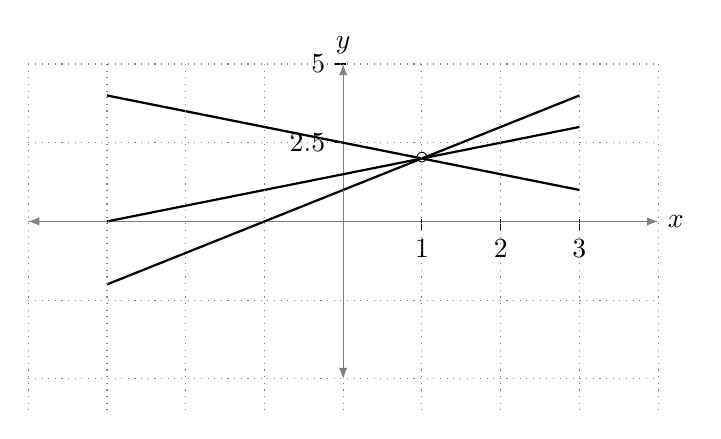
\begin{tikzpicture}[x=1cm,y=0.4cm]
    \draw[latex-latex, thin, draw=gray] (-4,0)--(4,0) node [right] {$x$};
    \draw[latex-latex, thin, draw=gray] (0,-5)--(0,5) node [above] {$y$};
    \draw[thick] (-3,-2)--(3,4);
    \draw[thick] (3,1)--(-3,4);
    \draw[thick] (3,3)--(-3,0);

    \foreach \Point in {(1,2.0)}{
      \node at \Point {$\circ$};
    }

    \foreach \x in {1,...,3}
      \draw (\x,1pt) -- (\x,-3pt)
        node[anchor=north] {\x};
    \foreach \y in {2.5,5}
      \draw (1pt,\y) -- (-3pt,\y) 
        node[anchor=east] {\y}; 

    \draw [dotted, gray] (-4,-6) grid (4,5);
  \end{tikzpicture}
  \caption{Shamir's Secret Sharing: with $t-1$ points known, there are still infinite solutions}
\end{figure}

In the sense of secret sharing $n$ would be any number of distinct points on
the generated polynomial, except the intercept with the value axis, which is
the secret.

The smallest degree of a polynomial, that is not a single point, is a line, a
polynomial of degree 1, it therefore be reconstructed with two points. It
consequently creates an edge condition of $t \geq 2$.
\cite{how_to_share_a_secret}

\subsection{Blakley's scheme}

Blakley's scheme offers another but referring to the idea quite similar
approach for secret sharing. For a secret which consists of two parts, 
Blakley encodes the parts into two dimensional, non-parallel linear functions.
The point where the graphs of the two functions intersect represents the
secret. For example, if the secret $s$ is $4$, one has to compute two non-parallel
linear functions intersecting at $y = 4$. It is simple to generate those two
functions if one remembers how to compute the point of intersection of two graphs.

For 2D graphs, the intersection can be computed by equating one function with
another function:

$$f(x) = g(x)$$

The standard linear function is $f(x) = mx + b$ where $b$ is the y-intercept and
$m$ is the slope. Two functions are considered parallel if their slope $m$ is 
the same. So now, a more formal definition of two nonparallel lines (which are
always intersecting) is the following:

$$m_1x + b_1 = m_2x + b_2$$

Now, resolve after x:

$$m_1x - m_2x = b_2 - b_1 $$

$$x (m_1 - m_2) = b_2 - b_1$$

$$x = \frac{b_2 - b_1}{m_1 - m_2}$$

Since $b_1$ and $b_2$ as well as $m_1$ and $m_2$ are constants, we can simplify

$$x = \frac{B}{M}$$

To now encode a secret with two parts, one simply has to generate a number $B$
and a number $M \neq 0$ whose quotient is $s$.
$B$ can then be split into $b_1$ and $b_2$ at will
while $M$ has to be split as well, but $m_1 \neq m_2$ (non-parallel lines).

If one instead wants to split a secret for three participants, one has to
create three planes. The point where the three planes intersect
is the secret point (as seen previous for secrets with two participants).
A line can be described by a slope and an intercept. A plane has one
additional ``slope'' which then spans up the plane. For each further
dimension, an additional component is needed. As a result, the space needed
to describe such planes or more general, hyperplanes, rises with the
threshold of needed participants in a shared secret.

\cite{blakley1994linear}

\subsection{Choosing a scheme}

Both secret sharing algorithms achieve security and are able to produce
parts which can be shared across several participants. Blakley's scheme
has the important drawback of larger shares the larger the threshold (number
of needed persons to recover a secret) becomes. It can be limited using
several techniques but that would increase the complexity of the encryption.
As a result, a space efficient and for the use case of duse optimal secret sharing
scheme is \textit{Shamir's Secret Sharing} due to it's simplicity and
security.

\section{Practical Secret Sharing}

The math behind secret sharing schemes has been proven long ago, however, for a
human to use a secret sharing scheme practically some additions have to be
made.

Those include:

\begin{itemize}
  \item cryptographic security
  \item using text instead of numbers
  \item correctly handle random values
\end{itemize}

\subsection{Finite Fields}

To be cryptographically secure, the operations are to be done within finite
fields. Using Shamir's Secret Sharing scheme that means, that the prime of the
finite field has to be larger than the secret integer. $P > S$

To get such a prime number, one has to test numbers larger than $S$. For example
for the number $S = 25$, the prime number $P$ would be $29$. In that case it is
easy to get a prime number, but for larger numbers it takes a lot of time to get
the next prime number. That's why one needs to have a more efficient method of
getting large prime numbers in a small amount of time.

To always have accurate prime numbers one has to either have a way to efficiently
calculate prime numbers as they are needed or a way to efficiently get a prime
number of a pre-computed set. Each prime number \textit{covers} its range. For
example, for a secret $S = 14$, the prime number $P = 17$ is suitable as it
\textit{covers} the range from $13$ to $17$. As a result, the range of each
prime number $P$ is from $P_{-1} to P-1$, where $P_{-1}$ is the next smaller
prime number. Data structures to organize range data exist, like for
example so called \textit{R-Trees}\cite{guttman1984r}. These are data structures
which are used inside database systems and can hold multidimensional data like
range rectangles. Since the needed datastructure would not store rectangle
bounded data but line bounded data, the R-Tree is inappropriate for this use.
But before inventing new data structures, one should first think of the space
requirements of the data to store:
If one tried to store the prime numbers from $0$ to $10^{100}$, one would need
an incredibly high amount of storage. As a result, the approach to store all
prime numbers in a datastructure is quite inefficient in terms of storage and
overall hard to realize.

While it is hard to identify the next prime larger than $S$, there is a
phenomenon that $2^p-1$, is likely to be a prime. These primes are called
Mersenne primes, with $p$ being the $p_{th}$ Mersenne prime. The largest known
Mersenne prime is the 48$_{th}$ and has $17,425,170$ digits.
\cite{largest_prime}

The only limitation is that $P > S$, so any prime larger that the
secret is valid. Using Mersenne primes we can easily use the known primes in
order to discover an appropriate finite field.

This, however, creates a new limitation. A secret can theoretically be larger
than $17,425,170$ digits. To avoid using the secret sharing scheme with larger
secrets, it can be divided into several parts. This ensures that the limit
is never reached for a single part. Then the secret sharing scheme is applied to
each part instead once per secret.

Fortunately this also has another side effect. If the secret and thus the
calculated shares could be infinitely long, then they would be very inefficient
to persist and process. Splitting allows the data to be processed sequentially,
in a stream. One large secret or shares would require one long loading and
processing operation.

\subsection{Euclidean algorithm}

The euclidean algorithm was discovered by Euclid, a Greek mathematician and it
determines the greatest common divisor of two numbers.
Hence it is often referred to as \textit{gcd}. There are several variants
of the euclidean algorithm, the \textit{classical} euclidean algorithm and the
\textit{modern} variant of it.

\subsubsection{Classical euclidean algorithm}

Euclid used the property that the greatest common divisor of two numbers does
not change if the larger number is subtracted by the smaller number. The classical
algorithm in iterative form is described in listing \ref{code:euclid_classic}

\begin{lstlisting}[caption={Classic euclidean algorithm}\label{code:euclid_classic},captionpos=b]
EUCLID-CLASSIC(a, b)
  if (a == 0)
    return b
  while (b != 0)
    if (a > b) // Determines larger side
      a = a - b
    else
      b = b - a
\end{lstlisting}

\subsubsection{Modern euclidean algorithm}

If the difference between the two numbers is large, the classical algorithm
needs many subtraction steps until termination. The modern euclidean algorithm
addresses these problems by applying modular divisions instead of subtractions.
It starts of with $a$ and $b = r_0$, the first remainder. The algorithm then
proceeds as described in listing \ref{code:euclid_modern}. It continues to
calculate the remainder $r$ until it is $0$.

\begin{lstlisting}[caption={Modern euclidean algorithm}\label{code:euclid_modern},captionpos=b]
EUCLID-MODERN(a, b)
  while (b != 0)
    h = a mod b
    a = b
    b = a
  return a
\end{lstlisting}

\subsubsection{Extended euclidean algorithm}

While the regular versions of the euclidean algorithm calculate the greatest
common divisor $gcd(a, b)$ of the two numbers $a$ and $b$, the extended
euclidean algorithm additionally calculates the numbers $s$ and $t$ so
that $gcd(a, b) = s \cdot a + t \cdot b$.

It proceeds by first calculating the regular euclidean algorithm. In each
step, the current $a$, $b$ and $q$ are saved into a matrix. $q$ is the division
result of $a \Mod b$. For each row, one now has to calculate
$g = s \cdot a + t \cdot b$, where $g = gcd(a, b)$. The calculation begins from
the last line, bottom up. For the last row, $s = 1$ and $t = 0$. For each
following rows, $s = t_{old}$ and $t = s_{old} - q \cdot t_{old}$.

\cite{cormen2001introduction}

\subsection{Polynomial interpolation}

The polynomial interpolation tries to find a polynomial of maximum degree $n - 1$ which
contains $n$ given points. Several algorithms exist which solve this problem,
the most famous of them being the so called \textit{Lagrange Interpolation}. The
Lagrange interpolation takes these $n$ points and transforms them into \textit{Lagrange
polynomials}. The formula for a Lagrange polynomial is

$$l_j(x) = \frac{(x - x_0) \cdot (x - x_1) \cdot \ldots \cdot (x - x_{j - 1}) \cdot (x - x_{j + 1}) \cdot \ldots \cdot (x - x_n)}
{(x_j - x_0) \cdot (x_j - x_1) \cdot \ldots \cdot (x_j - x_{j - 1}) \cdot (x_j - x_{j + 1}) \cdot \ldots \cdot (x_j - x_n)}$$

where $j$ is for each point from $0$ to $n$. This formula can also be put short with:

$$\prod_{s = 0 \wedge s \neq 0}^{n} \frac{x - x_s}{x_j - x_s}$$

These Lagrange polynomials are then put together as follows:

$$p(x) = \sum_{j = 0}^{n} y_jL_j(x)$$

\subsection{Secretly Sharing Strings}

While secure secret sharing schemes work with numbers, secrets generated by
humans are generally strings. Accordingly the schemes must be extended to
support strings.

One solution to the problem is to only allow a specific set of characters. Take
ASCII for example. ASCII has 128 characters. To convert a string to an integer
in a way that is reversible start with a result of 0. Process each character of
the string from left to right one at a time. Multiply the current result with
the length of your set of characters for every character in the string and add
the position of the current character in your set of characters, also known as
a code point. (see listing \ref{code:stringToInteger})

\begin{lstlisting}[caption={Converting an ASCII string to an integer}\label{code:stringToInteger},captionpos=b]
STRING-TO-INTEGER(input)
  result = 0
  while char = next-character(input)
    // 128 is the length of the ASCII Charset
    result = result * 128 + CODEPOINT(char)
  return result
\end{lstlisting}

\textit{DIVMOD} is the inverse function to what was applied to each of the
characters. \textit{DIVMOD} can be seen as a mathematical operation returning
two results. One of the results would be the same as if the modulo operation
was applied and the other the result of integer division.

To reconstruct the string using \textit{DIVMOD}, all that has to be done is
apply \textit{DIVMOD} to the input integer and use the result of the integer
division for the next iteration and the remainder of the modulo operation is
the code point of the next character. The string is reconstructed from left to
right. (see listing \ref{code:integerToString})

\begin{lstlisting}[caption={Converting an integer to an ASCII string}\label{code:integerToString},captionpos=b]
INTEGER-TO-STRING(input)
  result = ""
  while input > 0
    // 128 is the length of the ASCII Charset
    input, codepoint = input DIVMOD 128
    result = CHAR-OF-CODEPOINT(codepoint) + result
  return result
\end{lstlisting}

One of the challenges of secretly sharing strings however, is to support a wide
range of characters. As a result ASCII is not very effective since it limits
the characters immensely, which is a result of ASCII being created to display
only the English language. An encoding, which supports a large set of
characters and is widely used is UTF-8.

Since UTF-8 has a very large set of characters (1114112 to be exact) simply
converting all characters as explained is impractical. To allow the usage of
UTF-8 anyways the easiest solution is to encode the UTF-8 strings as Base64,
then apply the string to integer conversion as explained using the ASCII
charset. This is possible, since all characters of Base64 are a subset of
ASCII. \cite{unicode_spec}

\subsection{Correctly using random values}

Most languages provide a way to generate cryptographically secure random
values, however, even when using these methods, there are still a number of
possibilities to incorrectly use these random number generators.

Built-in random number generators often allow specifying an upper bound to
randomly select from. The result is a number between zero and that upper bound.
Specifically in the case of Shamir's Secret Sharing, when a random polynomial
is generated, the coefficients should not be zero. If a coefficient is zero, it
can potentially result in a lower threshold than intended. Say the randomly
generated polynomial is of degree three and in standard form. A polynomial of
degree three has a threshold of four.

$$f(x) = a_0 + a_1 * x + a_2 * x^2 + a_3 * x^3$$

If $a_3$ were to become zero through the random number generator, then the
threshold would suddenly be three instead of four. To avoid this, the
coefficients randomly selected must be greater or equal to one and smaller or
equal to the selected prime.

$1 \leq a \leq p$

\subsection{Share representation}

How Shamir's Secret Sharing can be extended to use finite fields and allowing
UTF-8 have been discussed. To communicate a share, however, a reasonable string
representation has to be chosen.

The main components of a Shamir's Secret Sharing share are the \textit{x} and
the \textit{y} value. Combining them in a single string can be accomplished by
concatenating the two around a dash. While the \textit{x} values will only
become as large as the number of participants, the \textit{y} value can become
any number up to the chosen prime. Since the shares are not human readable,
the \textit{y} value can be compressed by turning them into hex representation
instead of decimal.

Also, to be able to predict the length of a share better, the \textit{x} value
will have a left padding of zeros. If the number of participants is represented
by $n$ then the length of \textit{x} with zero-padding must be
$floor(log_{10}(n))+1$. For example, there are ten participants, then

$$n = 10$$
$$floor(log_{10}(n))+1 = 2$$

Accordingly, the \textit{x} values are represented as $01, 02, 03, 04, 05, 06,
07, 08, 09, 10$.

An example of the explained representation could be \textit{"1-f0"}, which is
equivalent to the point $(1, 240)$.

Additionally the representation is in use by other Shamir's Secret Sharing
libraries, therefore compatibility is more uncomplicated when choosing the
argued representation.

\subsection{Connecting Shamir's Secret Sharing and RSA}

When using Shamir's Secret Sharing, even under consideration of finite fields,
an attacker can estimate the size of a secret since it is somewhat close to the
chosen prime. To eliminate this possibility and introduce more security
features such as integrity and authentication, Shamir's Secret Sharing and RSA
are going to be combined. Due to some limitations of both technologies some
adaptions have to be made. These mainly concern length restrictions of RSA.

When using an RSA public key to encrypt a plain text, the resulting length of
the cipher text is equal to the key size. In case of an 1024 bit RSA key, the
resulting cipher text is always 128 bytes. Within those 128 bytes are a minimum
of 11 bytes PKCS1.5 padding, which leaves up to 117 bytes of actual payload. As
discussed in the previous section the string representation of a share always
contains a dash, leaving 116 bytes. The \textit{x} value is also at least one
character, leaving up to 115 bytes of payload.

Since the chosen prime restricts the size of the shares \textit{y} value, it
has a heavy influence on the total size. To calculate the maximum size of the
payload, the primes have to be examined. The largest possible share can be
represented as only 15 or \textit{f} in terms of hex. Since the Mersenne primes
are used, they can be examined for their maximum size. The expected prime is
the Mersenne prime below the first prime resulting in more than 117 bytes.

$$11. Mersenne prime: 2^{107}-1$$
$$2^{107} = 800000000000000000000000000_{16}$$

$$12. Mersenne prime: 2^{127}-1$$
$$2^{127} = 80000000000000000000000000000000_{16}$$

$$13. Mersenne prime: 2^{521}-1$$
$$2^{521} = (2*10^{130})_{16}$$

Since the 13$^{th}$ Mersenne prime is the first one to exceed 117 digits in
hex, the searched for prime is the 12$^{th}$. Therefore the maximum length for
a single share can be up to 34, since the length of the \textit{y}
representation can be up to 32 bytes. The two additional bytes are for the
dash, and at least one byte for the \textit{x} value representation.

$$floor(log_{10}(80000000000000000000000000000000)) + 1 = 32$$
$$length(x) >= 1$$
$$length(y) = 32$$
$$1 + length(x) + length(y) = total\_length$$
$$1 + length(x) + 32 = total\_length$$
$$1 + 1 + 32 <= total\_length$$
$$34 <= total\_length$$

\chapter{Quality Assurance}

Quality assurance in software covers all aspects of a software's life cycle.
From design over the process of development, code revisions, testing and
deployment.

To ensure the best quality software, metrics and practises are applied.

\section{Testing}

Tests help to ensure the software meets the requirements and identify bugs.

Testing is an integral part of software development. Today this is especially
the case for test automation. As software becomes more complex it is not
feasible to manually test an application. Most tasks are even to complex for
humans to perform, or they would take a lot of time and be error-prone.

There are several kinds of methods used in automated testing. Some of them
focus on the exhaustiveness of the overall testing, others to ensure that bugs
that already occurred do not appear again.

\subsection{Mutation testing}

While testing software is a widely adapted technique, the question is often,
how many tests and more importantly which tests to write. There are numerous
metrics describing the effectiveness of tests.

Mutation tests make sure the existing tests are exhaustive enough. To do so,
the productive code is mutated, hence the name. There are several mutation
techniques.

After each single mutations the tests suite runs and at least one test must
fail. If at least one test fails, the mutation is covered by said test.
Otherwise the mutation is remembered and the next mutation is applied. At the
end all uncovered mutations are listed for the developer to implement. This
method helps developers to test for boundary values, as they are often
automatically discovered by mutations.

Mutations include modification of conditions, literals, return values,
replacing objects with null references, deleting code, and many more, also
depending on the language used.

\begin{lstlisting}[caption={Mutation missed example}\label{code:bad_mutation},captionpos=b]
# production code
calc(float input)
  floor(input / 2)

# test
assertEquals(calc(4), 2)
\end{lstlisting}

In the case of integer literals being modified they could be modified by
increasing or decreasing it or setting it to another random value. Then a test
must cover whatever effect the value of the literal has and hopefully
invalidate that cause when it is modified.

Take listing \ref{code:bad_mutation}. While all lines and branches are covered,
there are mutations that are going to fail. For the specified asserts, the
\textit{floor} function is completely irrelevant. The mutation of removing the
call to the \textit{floor} would still make the test pass, therefore the
mutation fails. To eliminate this mutation, a test with an uneven number would
have to be added.

When using conditions, it happens easily that a condition is not properly
defined. Therefore mutating rational operators can be useful to determine the
correctness and effectiveness of the defined condition.

Similar to other metrics for tests it is usually very tedious to reach 100\%
mutation coverage, but it ensures that the present tests are as thorough as
possible.

There are mutation testing tools for some languages, but many lack their
presence.

\cite{mutation_testing}

\subsection{Regression testing}

Regression testing are known as tests used to discover bugs in existing
functional code bases, when adding new code, fixing code or modifying
configurations of any kind. These tests often originate from previous bug
reports.

Regression tests avoid, that previously patched bugs do not occur again. In
complex systems adding a new feature often results in breaking corner cases of
other features. When that happens regressions are there to tell the developer
about it. \cite{regression_tests}

Obviously these tests should be automated, for the developer to execute when
implementing new features or patches.

\section{Code Coverage}

Tests are great but they might be ineffective, test the wrong things
or simply are too few to assure no bugs. This is why there are metrics
for tests and other tools to test whether tests are effective or not.

\subsection{Branch Coverage}

One measure for tests is the so called \textit{coverage}. Coverage
comes in two flavors: The first one is the \textit{Branch Coverage}.
Branch coverage determines whether a test has run through the
required paths of a program. To calculate the branch coverage of a test,
simply divide the number of covered branches $c$ by $b$, where $b$ is the
total number of branches. For example, imagine the method listing \ref{code:branchCoverage}

\begin{lstlisting}[caption={abs method (calculates the abolute of an input number)}\label{code:branchCoverage},captionpos=b]
abs(int input)
  if (input < 0) return -input
  else return input
\end{lstlisting}

This method has got two paths: If the number is negative, it will
be multiplied with $-1$ to get the positive absolute of the number.
Otherwise (if it is already positive), it returns the original input.

Now imagine if one wrote the following test listing \ref{code:oneBranch}

\begin{lstlisting}[caption={One branch covered}\label{code:oneBranch},captionpos=b]
assert(abs(5), equals(5))
\end{lstlisting}

Of the two paths of the method, only the path with positive numbers is
covered. This leads to $c$ (the number of branches covered) being $1$,
as a result the branch coverage is $\frac{1}{2} = 0.5$. A test with
full branch coverage would be in listing \ref{code:fullBranch}

\begin{lstlisting}[caption={Full branch coverage}\label{code:fullBranch},captionpos=b]
assert(abs(5), equals(5))
assert(abs(-5), equals(5))
\end{lstlisting}

Full branch coverage is hard to achieve, but important for full testing.

\subsection{Line Coverage}

Another metric for test coverage is the \textit{line coverage}. The line
coverage determines the number of lines covered during a test. It is much
easier to get 100\% line coverage, but tests with 100\% line coverage do
not guarantee the absence of errors. \cite{bad_line_coverage}

\section{Continuous Delivery}

Continuous Delivery embraces test automation, Continuous Integration and the
continuous installation of a software product. It allows teams to perform task
with lots of agility while improving the software's quality.

A central concept of continuous delivery is known as the deployment pipeline.
The deployment pipeline is the collection of processes a software has to go
through before being released or deployed. An example of a deployment pipeline
could be: 

\begin{itemize}
  \item{run tests}
  \item{compiling the source to its targets}
  \item{packaging the application}
  \item{deploying the application to a staging environment}
  \item{executing acceptance tests}
  \item{deploying to a production environment}
\end{itemize}

The trigger for the deployment pipeline is often the used version control
system. Once a new revision is created and uploaded an automated mechanism
triggers the execution of the tests. All tasks trigger the next task once they
finish successfully. If any task fails, preferably the developer who caused the
error should be informed.

This approach allows easy rollback in case a faulty version passed the checks,
since earlier versions of the software can be deployed from version control.

Following this methodology allows teams to ship extremely early and often.
Accompanied by the perfectly fitting use of the so called Feature Toggle. A
Feature Toggle allows a developer to hide a feature, which is currently in
development, in production, but have it available in the other phases of the
deployment pipeline. For example the Feature Toggle is turned on in the staging
environment. It can be thought of as beta testing on a feature basis.

Integrating the deployment process into daily business of a developer reduces
the risks when deploying to the customer or production.

Continuous delivery does not only improve life for the developer, but also
allows customers to see results in very early stages of the development
process.

\cite{cd}

\subsection{Continuous Integration}

Continuous integration is the part of Continuous delivery ensuring that a
revisions changes are still allowing the automated tests to pass. The name
originated from the task of integrating all working copies from all developers
of a project. It ensures, that all code being produced still plays well with
the work from the other developers. Today the task of integrating is often done
with the version control system in use.

CI originated from the extreme programming methodology, however, today many
software teams embrace CI without following all extreme programming guidelines.
Typically CI is referred to as a server, service or platform where tests are
executed and the outcome is reported back to the development team. This is also
known as the feedback loop.

The benefits for a team applying Continuous integration are numerous. An important
benefit though is that the team eliminate the \textit{it works on my machine}
phenomenon. If the tests pass on the CI server, then the code is classified as
\textit{shippable}. It wipes out the possibility, that a local configuration,
the developer adds is lost along the way, which directly contributes to the
idea of continuous deployment. The CI becomes the central location of truth
concerning passing tests. \cite{cd}

\subsection{Code reviews}

Software teams regularly review their code to improve the software's quality,
reduce the risk of bugs and provide a consistent coding standard. Code reviews
can take place in different forms, but they all serve the same purpose.

A team can also perform code reviews through version control systems, without
requiring the team to be in the same place. These forms are referred to as
collaborative or crowdsourced reviews.

Code reviews have been researched and they show a significant discovery of
defects in software of 60 percent or more. In terms of continuous deployment it
is critical for a team to embed code reviews in their daily work to make sure
all code is reviewed. \cite{code_reviews}

\subsection{Blue green deployment}

A critical feature of continuous deployment is to deploy or release the
software in development several times a day. Feature toggles even allows
these systems to be run in production. Troublesome, however, is when end users
are restricted by downtimes of the application when deploying a new version to
production. To avoid end users ever noticing these downtimes, a method for zero
downtime has to be applied.

Blue green deployments allow deployments to be zero downtime. The approach is
simple. When deploying, there are two identical but separate environments. The
blue and the green environment. A router, in case of a web server this can for
example be a reverse proxy or a load balancer, decides to which environment a
requesting user is routed to. Before deployment the service points to the green
environment.

Assuming when the deployment starts, the green environment is live, then the
new version is deployed to the blue environment. In case something fails while
deploying, the router simply does not route to the blue environment. If the
deployment is successful, then the router switches to the blue environment,
thus the new version is now live without any downtime. (see figure
\ref{fig:blue_green_deployment}) Of course, this requires the router to hot-load the
new configuration.

\begin{figure}
  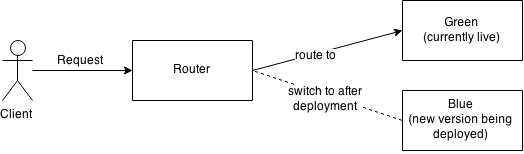
\includegraphics[scale=0.55]{pictures/blue_green_deployment.png}
  \caption{Blue green deployment}
  \centering
  \label{fig:blue_green_deployment}
\end{figure}

The two environments, blue and green, are often only used as a metaphor,
because the in the described case updated blue environment is created merely
for the deployment process. Once the deployment has been successful it is
viewed as the green environment and the now outdated environment is removed.
This approach leads to the thought of an immutable infrastructure, where the
philosophy is to never change the state of a deployed system and rather discard
it and fully redeploy it.

\cite{cd}

\subsection{Rolling updates}

Once applications receive more traffic, then multiple instances have to be
created and load balanced. In such an setting zero downtime deployments are
much easier, since there are already multiple instances of the application
running, there is no single point of failure. Once there is a new version to be
deployed, it is deployed one instance at a time. Since there are multiple
instances running anyways, there will be no noticeable downtime for end users,
thanks to the load balancer, which does not route to an instance that does not
respond yet. (see figure \ref{fig:rolling_updates})

\begin{figure}
  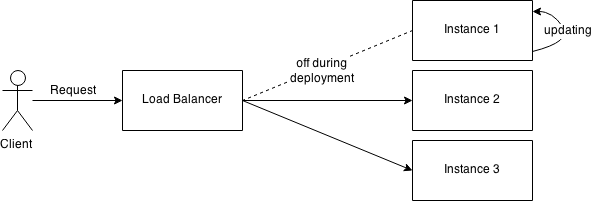
\includegraphics[scale=0.55]{pictures/rolling_updates.png}
  \caption{Rolling updates}
  \centering
  \label{fig:rolling_updates}
\end{figure}

While there is no established name for this method of zero downtime
deployments, it is sometimes referred to as rolling updates. \ref{rolling
updates}

\section{Dependency locking}

Even when keeping an eye on an applications technical dept, a few dependencies
will almost always exist. A problem with having dependencies is that they might
introduce breaking changes in the future, thus contributing to the projects
technical dept. To avoid complications with these possible breaking changes, a
method sometimes called dependency locking is used.

Dependency locking can be acted out in different ways, often depending on the
used language and tools. A popular approach is to have one file declaring the
projects dependencies with a possible restriction on minimum, maximum or exact
versions required. Once these dependencies are installed a new file, the lock
file is created. The lock file contains the exact version used by the
application. Using this method allows installs in any environment easier, since
version conflicts with locally installed version can be eliminated.

When new versions of the dependencies are released, updates can be performed in
a controlled way, rather than whenever an install happens. Updating
dependencies in a not controlled way as described can lead to hard to debug
problems in different environment. Worst case would be in production.
\cite{dependency_locking}

\section{12 Factor Apps}

12 Factor Apps is a set of rules to follow when developing web applications
developed by experts from Heroku. The rules provide a framework to make the
development of web applications maintainable, of high quality, and scalable.
Portability and agility of development is of high importance as well. As the
name states, there are twelve factors to consider when developing.
\cite{12factor}

\paragraph{Codebase}

When developing, the codebase is always revisioned using a version control
system. Any deployment originates from version control. Each codebase results
in a single application. A system of multiple applications can still be 12
Factor compliant, when each component itself is a 12 Factor app.

While there is only one codebase for each application, there are multiple
deployments of each application. There can be different stages between
development and release. Deploys are any running instance of the application,
even an instance running on a developers machine, locally. It heavily
contributes to continuous deployment, as the application is tested in every
stage of the development life cycle.

\paragraph{Dependency Isolation}

All dependencies are to be declared by the application. The codebase contains
not only which dependencies to use, but also exactly which version to use. It
prevents unintended dependency updates, possibly breaking an application. 12
Factor apps do not rely on system-wide installed dependencies. Dependencies are
isolated within the applications environment. Isolation of dependencies and
their declaration are always bundled together.

All dependencies should be installable in the isolated environment, to achieve
minimal system requirements.

\paragraph{Config}
\label{para:12factor:config}

Configuration parameters are to be stored within environment variables. It
allows the app to be configured by its environment rather than configuration
files, which would have to be checked into version control. As this is not
desirable the configuration is solely done by environment variables, or
configuration files generated by the environment upon deploys.

\paragraph{Backing services}

Any service an application relies on is a backing service. Backing services can
be message brokers, databases, caches and many more. All access details,
credentials and the location of these services are to be configured as
described in config. The importance is, that this allows these service to be
easily replaced in case of any incidents. All that has to be done, is
reconfigure the location of a backup service in the environment variable and
reboot the application.

\paragraph{Build, release, run}

Any change to a production system can only be done by changing the code locally
and create a new revision in the version control system to trigger a deployment
pipeline. No code is changed directly in a production environment. All
deployments are automatic, and in case of errors during a new deployment, there
is the possibility to rollback to the latest working version. To enable
rollbacks, every release has a unique identifier to refer to when rolling back.
There are various tools to support these intentions out of the box.

\paragraph{Processes}

Processes within an application are stateless. Stateful information is stored
and saved in a shared backing service. The backing service is in turn
responsible for keeping consistency, uptime and safety.

At all times it must be assumed, that a disk or memory is wiped or not
accessible. For example when an application is accessed no information is
stored on disk or in memory between subsequent requests as these requests might
not be routed to the same instance of the application.

\paragraph{Port binding}

12 Factor apps are completely self contained and bind the service they offer to
a specific port, which is configurable. Their runtime does not need to be
injected into a web server or otherwise. The application itself provides a
web server.  Therefore when running the application everything is executed in
the same user space and is not able to access unauthorized content due to
permissions.

The exposed service does not necessarily need to be HTTP, it can be any
protocol, and therefore a Backing service for other apps.

\paragraph{Concurrency}

Processes are used to scale the application. When respond times are decreasing
due to load on single instances, just add more processes to route to. An
application can consist of several types of processes. Each process has a
specific task to achieve. For example, there can be a process type responsible
for handling HTTP requests and one worker, handling long running background
jobs.

\paragraph{Disposability}

Disposability describes the value of a single instance in the whole
infrastructure of an application. Any instance can be started or stopped at any
time. A goal is to make this as efficient as possible, to be able to move
processes from one server to the other. Thus fast start and stop times allows
moving of processes to be done quickly.

Stopping an instance is done by sending the SIGTERM signal to the process. It
should then try to gracefully shutdown. A graceful shutdown for a web
application is to stop binding to its port and thus refusing any requested
connection. The client should be built to retry if connections fail, and be
routed to another running instance.

Gracefully shutting down a worker stops the current job, and returns it to the
job queue to ensure a job is done by another worker.

Besides graceful shutdowns, an application should also be built to tolerate non
graceful shutdowns as they can also occur due to hardware failure.

\paragraph{Development - Production parity}

Many bugs occur due to the parity between production and development. To avoid
this three things have to be minimized:

\begin{itemize}
  \item{Time between development to production deployment}
  \item{Different people developing and deploying}
  \item{Different tools used, such as different database technologies}
\end{itemize}

Minimizing these factors allows development to be as close to production as
possible and therefore minimize the risk of unintended behaviours in
production.

\paragraph{Logs}

Logs are viewed as streams of events. Storage of an applications logs is
transparent for it, the application simply prints its logs to stdout, which can
be captured by the environment running the application. It allows logs to be
handled completely separately. Since logs are a stream of events of the usage
it can be analyzed. Analyzing the usage can lead to the discovery of trends and
possibly generate alerts.

\paragraph{Admin processes}

While it is not allowed to change code in production, which should not be
possible anyways, sometimes it is necessary to run single commands in a
production environment, for example to receive insight of the data in the
database. Commands executed should run under the exact same environment as the
production code - same configuration, same environment variables, same
permissions. Even if code is of administrative use, it may not be added in
production without undergoing the deployment pipeline.

\chapter{Duse}

The most important part of a system to securely share secrets is the
cryptographic protocol consisting of multiple cryptographic primitives and
other protocols or algorithms. Since it is a security concerned system,
possible attacks must also be examined.

\section{The Cryptographic Protocol}
\label{sec:duse:crypto_protocol}

The protocol involves a server and a client. During a secrets life cycle, there
are four events that are relevant for the protocol creating, reading, updating,
and deleting. These are also known as \textit{CRUD}. Most interesting of those
are creating and reading a secret, because deleting just removes all related
data and updating essentially works like creating.

\subsection{Creating a secret}

When creating a secret, the client first has to retrieve all profiles of the
users the secret should be shared with. These profiles contain the public key
of each user.

Now Shamir's Secret Sharing could be used to split the secret into shares for
each user, however, this can lead to problems. Since Shamir's Secret Sharing
requires primes equally large as the input, it can in theory handle any size of
input, but not in practise, as it might take a long time to calculate such a
large prime. Instead the original secret is split into chunks, here called
\textit{secret parts}.

Considering that all the \textit{secret parts} are not too long to compute
primes for each of them, Shamir's Secret Sharing can now be applied.

Once Shamir's Secret Sharing has been applied there are shares for each user
for every secret part. These shares can then be encrypted with the previously
retrieved public keys of each user and then signed with the creating users
private key. All of this data is then sent to the server to verify and save.
(see figure \ref{fig:creating_a_secret})

Shamir's Secret Sharing requires at least two shares to reconstruct a secret,
therefore there will always be a transparent "server"-user which gets a share
that is shared with every participant. This is save, because the server does
not have access to any other shares, and a single shares does not reveal
anything about the secret.

\begin{figure}
  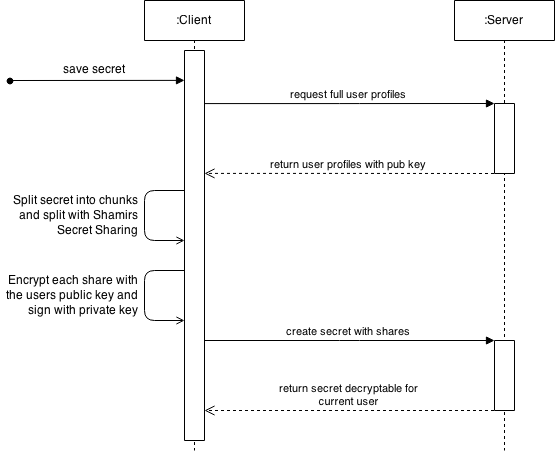
\includegraphics[scale=0.55]{pictures/create_secret_sequence_diagram.png}
  \caption{Creating a secret}
  \label{fig:creating_a_secret}
\end{figure}

\subsection{Retrieving a secret}

Retrieving a secret can be divided into two main parts, server and client
processing.

When a client requests a secret, the servers shares are first decrypted and
then encrypted with the requesting user's public key. The shares and additional
metadata, such as the secret's title and a list of participants, is then
returned as the response to the client's request.

Once the client received said response, it decrypts the shares and reconstructs
the secret parts using Shamir's Secret Sharing. Next the secret parts are
concatenated, and the secret is successfully retrieved.

\begin{figure}
  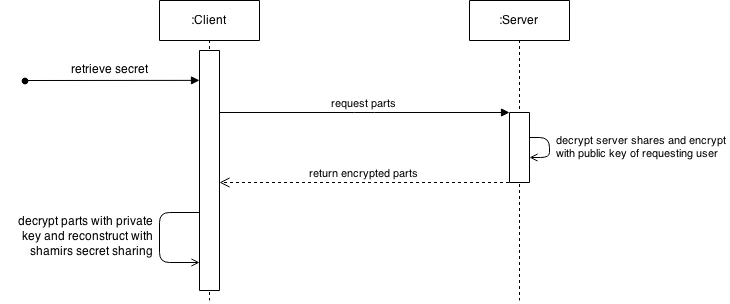
\includegraphics[scale=0.55]{pictures/retrieve_secret_sequence_diagram.png}
  \caption{Retrieving a secret}
  \label{fig:retrieving_a_secret}
\end{figure}

\section{Attacks}

Since this is an attempt to build a system to securely share secrets, possible
attacks must be examined. To prove the security of a protocol the Dolev-Yao
model is often used. The Dolev-Yao model includes abilities one must assume
when evaluating a cryptographic protocol. These include, that the attacker can
listen to all communicated messages, modify them and possibly send them to a
different recipient than the sender intended to. This essentially describes the
classic \textit{Man in the middle} attack. \cite{dolev_yao}

To validate the system further, the consequences of a completely compromised
system are examined.

\subsection{Man in the middle}

The developed cryptographic protocol has two essential elements, creating and
retrieving a secret. To evaluate the security of these components it is
assumed, that an attacker could modify all data exchanged from client and
server.

\subsubsection{Creating a secret}

There are several requests during the creation of a secret. The attacker cannot
decrypt the encrypted shares, however, the attacker could intercept when the
client requests the user profiles to share the secret with.

The attacker can replace the genuine public keys with its own counterfeit keys.
Then the attacker can decrypt the encrypted shares since the attacker knows the
matching private keys.

The described attack can be weakened when introducing a Public key
infrastructure. Then the clients can verify the authenticity of the received
public key.

There is a second aspect to be examined when creating a secret. The attacker
cannot create modified secrets, since the authenticity through RSA signatures
is checked upon receiving by the server. The attacker is only able to modify a
secret and save it, if the attacker had modified the public key, when the user
was created. To eliminate the possibility of such an attack the operator of the
system could use a second way of checking the authenticity of a users public
key, an eligibility check for example.

\subsubsection{Retrieving a secret}

Unless an attacker already modified the requesting user's public key, at time of
creation of the said user, then the attacker cannot determine the original
secret.

All shares are encrypted with the requesting user's public key, thus the shares
are of no use for an attacker, under the condition, that the key establishment
is secure.

\subsection{Compromising the server}

Once the attacker has compromised the server, the abilities match those of the
\textit{Man in the middle} attack, however, with the addition of access to the
database.

Fortunately an attacker cannot decrypt any share, since the users private key
is required to achieve that. Hence any of the stored shares, unless the
attacker previously already tampered the communication of a users public key at
time of user creation is useless for the attacker.

The only assumption an attacker can track is the circumstance, that a secret
has been divided into multiple parts. The number of parts can be used to
approximate the total length. All parts have a maximum length, thus the
attacker can multiply the maximum length by the number of parts and receives an
approximate length of the secret.

$$n: number\,of\,parts$$
$$l: maximum\,length\,of\,secret\,part$$
$$(n - 1) * l \leq length(secret) \leq n * l$$

\chapter{Technology basics}
\section{Web development}
\subsection{Middlewares}

Middlewares are a method in which software applications are built within
layers. Each layer only concerning the in- and output. It allows applications
to be more modular and increase the Separation of Concerns principle.

Within web development middlewares describe the architecture of a web server.  A
call to a web server is handled by several middlewares until one of the
middlewares produces and replies a response. Typically middlewares process
incoming data and then call the next middleware, until a middleware decides to
end the request and sends a response.

Middlewares can be used to authenticate a user and keep a request from entering
domain logic if not authenticated. A middleware could also transform the
request content to a unified form, for example parsing different text formats
and turning them into higher level objects, that way following middlewares do
not have deal with different format, and instead concentrate on its real
purpose.

\subsection{RESTful API}

REST is an abbreviation for Representational State Transfer. It describes the
behaviour of web services. It defines a set of constraints leading to several
advantages. It is usually practised via HTTP and its methods.

The constraints include

\begin{itemize}
  \item{Client-Server}
  \item{Stateless}
  \item{Cachable}
  \item{Uniform Interface}
  \item{Layered system}
\end{itemize}
\cite{rest_style}

\subsubsection{Client-Server}

This constraint is fundamental for any API as it tries to achieve
separation of concerns between client and server. It requires a client to be
completely independent of how resources are handled by the server. The server
should even be able to switch out technologies, without affecting the client.
This could for example be the replacement and migration to another database
management system.

The communication between server and client is to be done via a predefined
interface. Pervasively doing this allows multiple compatible servers and clients
to be developed simultaneously since they only have to develop against the same
specification.

\subsubsection{Stateless}

Statelessness is crucial for RESTful application to scale. Statelessness
requires the server to know nothing about a state of a user. All necessary
information to process a single request is also packaged within this one
request. Doing so allows the operator of the service to seamlessly add more
instances of the application without having to worry about synchronizing states
among them. For all instances of an application to still be synchronized in
terms of resources, they have to access a shared resource, such as a database
or cache server.

\subsubsection{Cachable}

Most web clients are able to cache data they receive, however, the server has
to tell when the data is cachable. There are multiple mechanisms included in
HTTP to make use of this. The server also has to tell the client what to use to
detect expired cache contents. Not only does caching reduce load on the server, but
it also allows clients to respond much faster, since they do not have to wait
for the server's response.

\subsubsection{Uniform Interface}

The uniform interface constraint is essential for a RESTful architecture. It
allows parts of a system to mature independently while only having to develop
against a specification.

Resources are identified by the request of a client. The request also indicates
which representation the client expects. The server keeps its own representation
and transforms the resource into the requested form.

Whenever a resource is requested or responded, it includes metadata such as its
representation for the other participant to know which representation is used
and parse it correctly.

Additionally a client has all required data to create, modify or delete a
resource.

Lastly, the Hypermedia as the Engine of Application State principle should be
applied. A resource has to be self explanatory as in which actions can be
applied, and which resources it is connected to. However, it does not nest the
connected resources in its representation, it only tells the client where to
find said resource. HATEOAS allows the viewed action's server to vary based on
the state of the data. This can be useful if a process requires multiple
requests to complete.

\subsubsection{Layered system}

It is transparent for a client accessing a service. The client can either be
directly routed to the actual instance of the application or a request can go
through multiple layers of caches and load-balancers. Combined with the other
constraints it might not even require a request to be routed to an instance of
an application at all, for example if a request is cachable and an expiration
date has been provided by the application, then a cache server could answer the
request without putting any load on an applications instance.

\subsubsection{REST Maturity Model}

There is a REST Maturity Model describing how consequent the constraints are
applied. It is very much scoped on web services using the REST principles via
HTTP. There are four levels, 0 to 3.

Level 0 describes services using XML-RPC or SOAP. These services are always
requested on the same identifier and only use a single HTTP method.

While level 1 also uses a single HTTP method, it differentiates by using
different identifiers and resources.

Level 2 is similar to level 1, but makes use of multiple HTTP methods.

In addition to all requirements for level 2, level 3 requires a service to
navigate using HATEOAS provided information.

\cite{rmm}

\section{Git}

Git is a distributed version control system initially developed in 2005 to
maintain the Linux kernel. Git uses, unlike other version control systems,
snapshots instead of deltas to represent a new version. Whenever a new version
is created each state of every file is saved in a new snapshot. If a file was
unchanged, then only a pointer to the latest version is saved in the snapshot,
this reduces redundancies.

A typical Git workflow includes

\begin{itemize}
  \item{commiting}
  \item{branching}
  \item{merging}
  \item{tagging}
  \item{pushing}
\end{itemize}

Commiting is simply the creation of a new version from local changes. Git
distinguishes between three main sections of a project. The working directory,
or the files the developer actually changes. Once the developer is ready to
commit changes or part of the changes, they are \textit{staged}. This is called
the staging area. When the developer is satisfied with the staged changes,
they can be committed to the directory.

Branching and merging is a pain point of many other version control systems. Git
has first class support for both. Every commit, with a few exceptions, has one
or more parent commits. It indicates, which commit the commit is based of off.
Branching allows a project to have several paths of development simultaneously.
This way a main branch can always be stable, while other branches contain new
feature development or fixes. Once these branches have reached maturity, they
can be merged back into the main branch. When merging Git looks at the latest
commits of the branches to merge and tries to merge with multiple strategies.
If there are still conflicts, then these have to be handled by the developer
manually. Merging often results in an additional commit, the merge commit.

Tags are special pointers. They can be used to reference a specific commit in a
repository. They are commonly used to specify versions of a software.

Since Git is a \textit{distributed} version control system, every developer has
their own local copy of the repository. Thus the changes have to be uploaded,
once the developer is done with the changes and wants to provide them to the
rest of the team. This action is referred to as \textit{pushing} changes. The
receiving server then makes sure, that there are no inconsistencies. \cite{git}

Various Git integrations make a perfect fit for use in a deployment
pipeline.

There are many more features and characteristics that make Git special, but for
the use in this project the highlighted features are essential.

\subsection{Hooks}

An essential feature of Git in a deployment pipeline are hooks. There are
multiple hooks in Git's workflow. Git can essentially embed a shell script
before and after any event happening in the life cycle of a repository. This
works on the client as well as on the server side.

On client side this can be used to make sure, that code which is about to be
committed, follows all required coding guidelines or other quality assurance
measures. The team can be sure, that before committing the tests have passed,
static code analysis and other statistics have passed. This is known as the
pre-commit hook.

On the server side, it can be used to trigger the entire deployment pipeline.
It tells the build server, that there is a new version to test. The build
server can then decide what to do, depending on what changes have been
introduced. For example: Deploy the application to production, if a new version
has been created using git tags or deploy to staging if it was just a new
commit. This hook is known as the post-receive hook. \cite{git}

\section{Docker}

Docker is an open-source project providing operating-system-level
virtualization. It is used to isolate applications inside containers. To
achieve this, it uses the cgroups and kernel namespace features of the Linux
kernel. Therefore it is only possible to use Docker on a Linux distribution,
however, there are workarounds so users of other platforms are also able to
use it.

The company behind Docker describes it as follows

\paragraph{}{"Docker enables any application and its dependencies to be packaged up as a
lightweight, portable, self-sufficient container. Containers have standard
operations, thus enabling automation. And, they are designed to run on
virtually any Linux server."\cite{docker_quote}\newline}

While traditional virtualization technologies have used application level
virtualization, Docker utilizes operating system virtualization. It allows
Docker to use Kernel functionalities directly from the host system, which
an application level virtualization could not do.

Docker introduced various concepts for to automate the creation and use of
containers. When an application is packaged with Docker, a bash like language
is used to declaratively describe how the image should be built. Once an image
is built, a container can be created from it. This fits perfectly into the
notion of an immutable infrastructure. Whenever a new version of an image is
released, the containers are simply stopped and deleted, and new containers of
the new version are started.

\chapter{Development}

\section{Big Picture}

The big picture, see figure \ref{fig:big_picture}, has three conceptual actors:

\begin{enumerate}
  \item[Users] Users access the duse RESTful API via various
  clients (CLI- and web-clients are depicted). One user can use multiple
  clients and therefore is not bound to any specific client. The clients
  establish their connection to the duse API via HTTP calls on REST
  resources.

  \item[RESTful API] The RESTful API is the core of the
  duse application stack. It consists of four main components. The first
  component, the routing, takes care of routing calls to the correct
  resources. The syntactical correctness is ensured here(like checking
  for tokens or well-formedness etc.). The next layer is the organization
  layer. Here, the structure of the secrets as well as accessing them is
  controlled. The most inner layer is the data. These are the raw, public
  encrypted secrets which are accessed via an ORM on the database.

  \item[Database] Database access is highly abstracted inside an
  ORM. The database stores the various secrets in
  different tables. It is a relational database, but duse does not depend
  on any specific implementation. If there is an adapter for the ORM
  duse uses, the database can be used.
\end{enumerate}

\begin{figure}
  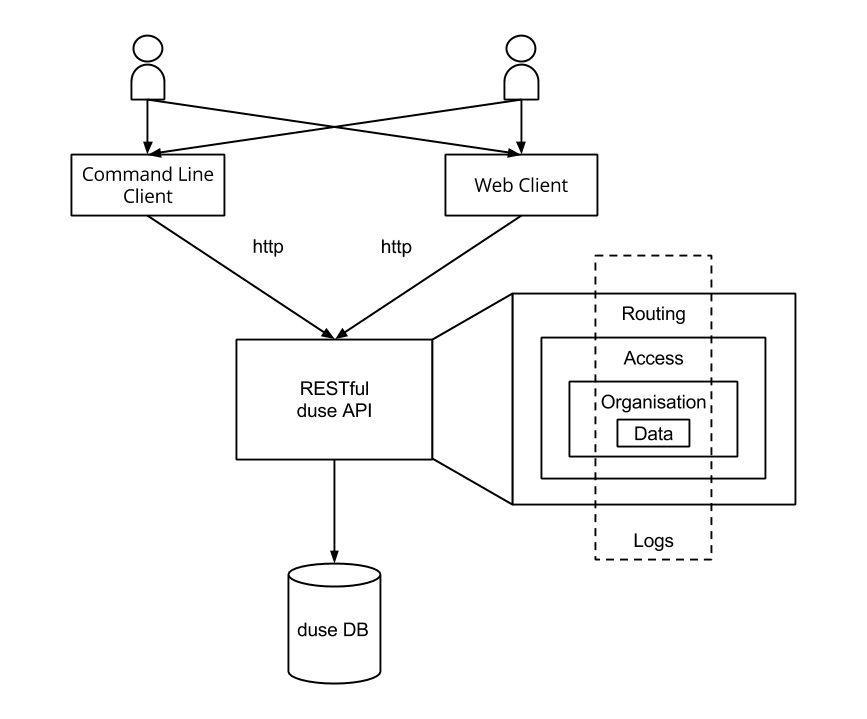
\includegraphics[scale=0.55]{pictures/big_picture.png}
  \caption{Duse Big Picture}
  \centering
  \label{fig:big_picture}
\end{figure}

\section{API}

Duse is a so called API first application. Meaning the software development
highlights building the components of a system as APIs. In the case of duse, it
is a central RESTful API. By embracing this, it is straightforward to create
several clients, cross platform and for multiple languages.

\subsection{Architecture}

Duse's RESTful API is composed of multiple middlewares.

When a client makes an HTTP request, the first middleware the request passes
through is a middleware enabling \textit{Cross Origin Resource Sharing}. This
is necessary for possible HTML front ends for the web browser. Web browsers have
the \textit{Same Origin Policy}, it forbids JavaScript, ActionScript and CSS
from accessing resources from another origin than the host which the browser
currently accesses. CORS has been introduced to relax the SOP. It allows the
configuration of possible access points. CORS can be restricted to specific
resources or resource patterns as well as specific HTTP Verbs. The web browser
performs the so called \textit{preflight}, which is an HTTP Options request. The
web browser then allows or denies the access, depending on the content of the
response. The said middleware handles the \textit{preflight} requests and
allows any resource to be requested with all HTTP Verbs.

If the request is not a CORS specific request it is passed on to the next
middleware, which is responsible for authentication. It deserializes a session
for direct access to the requesting user in the following program logic,
however, using sessions as in session-cookies is not appropriate for an API.
Session cookies would be a pain to scale when the API grows in instances, as
the session would be bound to a single instance. To avoid this and other pain
points, authentication tokens are introduced. Authentication tokens can be
created by providing username and password once. Requests require the
\textit{Authentication} header to be set with a previously retrieved token.
This token is then used to identify the requesting user. Additionally
authentication tokens could be restricted in the allowed actions, which can be
performed using it. For example a specific authentication token might be
read-only.

Once the request is through the authentication middleware, it is passed to a
version switch. The version switch is useful for multiple things. It examines
multiple aspects of the requests and decides which version of the API the
request is routed to. By default, it uses version one of the API, but it makes
future releases of the API much simpler. It can also be thought of as a feature
toggle, since future releases of the API can be developed and be turned of
until it has reached maturity and then the switch allows access to it.

After the version switch the request is passed to the appropriate version of
the API. Each version is essentially its own application.

Since CORS and authentication is already taken care of, the application can
purely focus on its purpose.

There are several endpoints for mainly two substantial ones, secrets and users.
User endpoints are not very interesting. They take care of user registrations,
confirmation and viewing users. The endpoints for secrets are a typical CRUD,
but involve several steps to complete. (see figure \ref{fig:action_flow})

In case a step cannot complete successfully, it returns an error code along
with an error message. Otherwise, the request is processed further by the next
step, which can now assume the past steps have been successful.

\begin{figure}
  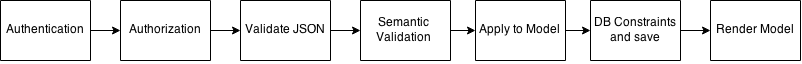
\includegraphics[scale=0.50]{pictures/action_flow.png}
  \caption{Action Flow}
  \centering
  \label{fig:action_flow}
\end{figure}

Error conditions for the steps are as followed (see table
\ref{tab:error_codes}). Successful responses describe, how the resource has
changed. (see table \ref{tab:success_codes})

\begin{table}
  \begin{tabular}{|l|l|l|}
    \hline
    Step & HTTP Codes & Description \\ \hline
    Authentication & 401 & No or invalid authentication \\ \hline
    Authorization & 403 & Insufficient permissions to perform the action \\ \hline
    JSON Validation & 400, 422 & \parbox[t]{10cm}{HTTP 400 code on malformed JSON\\HTTP 422 code when the JSON does not match the schema} \\ \hline
    Semantic Validation & 422 & Data did not pass the semantic criteria \\ \hline
    Apply to Model & 422 & Database constraints are not met \\ \hline
  \end{tabular}
  \caption{HTTP Error codes with description}
  \centering
  \label{tab:error_codes}
\end{table}

\begin{table}
  \begin{tabular}{|l|l|l|}
    \hline
    Action & HTTP Codes & Description \\ \hline
    Create & 201 & a new resource has successfully been created \\ \hline
    Read & 200 & Resources unchanged, only read \\ \hline
    Update & 204, 200 & \parbox[t]{9cm}{HTTP Code 204 If Resources are left unchanged\\ HTTP Code 200 If the change was successful} \\ \hline
    Delete & 204 & Deletion of the resource has been successful \\ \hline
  \end{tabular}
  \caption{HTTP Success codes with description}
  \centering
  \label{tab:success_codes}
\end{table}

\section{Validation}

Validation of data coming into the system is complicated especially for the
nested structures of secrets. To prevent unnecessary load on the server when
validating the data itself, the structure of it is validated first.

\subsection{Structural Validation}

The most popular representation of data in RESTful APIs today is JSON. It only
has a small amount of metadata.

There are multiple approaches to validating JSON, however, they actually do not
rely on JSON. It is rather a structural validation, applied to JSON.

A possible approach, can be to reduce the JSON in the request body to a
predefined set of attributes, and apply what is left directly to a model. The
model then verifies itself and saves to the database.

Another approach is to define a schema, which the JSON is verified against. The
JSON schema draft describes such an approach. It can be used to extract,
validate structurally and partly to validate the content. Content can be
validated by providing the expected data type or a regular expression. Data types
include the JavaScript primitives: Integers, String, Array, Object, Float.
Furthermore it provides more complex types such as email, IP-Address,
date-time, URI, and hostnames. \cite{json_schema_draft}

After the validation of data types, the schema can also define some semantic
validations, such as constraints on numbers or length of a string, however,
these validations fail in its effect to validate relations between nested
entities.

Not only does JSON Schema allow validation, but it also leaves the database
untouched until the data is in the correct format. Besides ensuring the correct
format of the data, it also has straightforward documentation advantage. Since
the JSON Schema is written in JSON itself, it can easily be published to
informs users of the API about the correct usage, instead of single possibly
misleading examples.

A weakness of existing implementations of the JSON Schema draft are error
messages. An error message often looks like the following

\paragraph{}{"The property '\#/a' of type String did not match the following type: integer in
schema 03179a21-197e-5414-9611-e9f63e8324cd\#"}

\paragraph{}{While it accurately states the situation, a more descriptive message would be
appropriate for users not aware of the use of JSON Schema, since the schema
UUID is not relevant for the single property.}

\paragraph{}{ 
  
  The JSON schema for a secret can be modeled as in listing
  \ref{code:secret_JSON_schema}. At top level, it expects an object. This
  object has two properties, a title and parts. Parts are an array of arrays
  containing the shares. A share is represented by the user it belongs to, with
  the \textit{user\_id}, the encrypted content and the signature to verify the
  author of the secret.

}

\begin{lstlisting}[caption={JSON Schema of a secret}\label{code:secret_JSON_schema},captionpos=b]
{
  "type": "object",
  "required": ["title", "parts"],
  "properties": {
    "title": { "title": "string" }
    "parts": {
      "type": "array",
      "items": {
        "type": "array",
        "items": {
          "type": "object",
          "properties": {
            "user_id": "integer",
            "content": "string",
            "signature": "string"
          }
        }
      }
    }
  }
}
\end{lstlisting}

\subsection{Semantic Validation}

When creating or updating a secret, the input can very well comply with the
JSON Schema, but are not valid to be saved to the database. More specifically,
the parts and shares must be validated. Each part contains shares, which in
turn contain a users id, the shares content encrypted with the associated users
public key and a signature created by the user performing the action.

All of the shares in a single part can be correct in terms of the structural
validation, but still be incorrect. The user referenced by its id in a share is
simply an integer in the schema, but incorrect, if the user does not exist.
Even though the content of the share cannot be verified, that its decrypted
content is valid, it does have some constraints, which can be applied. Since
the share is encrypted with the users public key, the contents length must be
equal to the size of the users public key and only contain base 64 compatible
characters. The signature also has to be verified against the users public key
performing the action.

Once each single part is verified, all parts together must be verified. Each
part has many shares. Each part must contain shares for the same set of users,
for each part the users must also be unique. Furthermore, there must always be
a share belonging to the server and a share for the user performing the current
action, to avoid the possibility of creating secrets for other users. At last,
to prevent pollution of the database by users, the number of shares can be
restricted.

\section{Clients}

\subsection{Shamir's Secret Sharing Library}

While there are libraries available for cryptographic primitives in most
languages, Shamir's Secret Sharing is not as widely spread. Therefore it has
to be implemented for the used technologies.

To ensure, that the cryptographic libraries are thoroughly tested, mutation
testing is applied, where the tooling is available.

\subsection{Web front end}

As every modern computer has got a browser as well as an internet connection today,
a web front end was a requirement from the beginning. This web front end should be
easy to use but offer the same security and the same features as the command line
client does. An issue of many of today's browsers is their support for
cryptographic operations which conflicted with the security requirement:
Since duse uses a lot of random numbers, random number generation is an important
security aspect. Inside the command line client, randomness sources such as
/dev/random could be used but not all modern browsers offer such randomness
sources. Therefore a strong but also slower pseudorandom number generator has
to be used for the web front end.

The web front end is built in a language which runs inside a virtual machine and
can also be cross-compiled to the web's lingua franca JavaScript. As a result,
the library for the web front end can also be used to implement an
additional command line client (which wasn't the focus during implementation).

\subsubsection{Issues and Mitigations}

As the programming language used inside the front end technology is relatively
new (it was first unveiled in 2011), its ecosystem is rather small. Many
important functionalities have to be implemented by hand. Quality assurance
and cryptography functions belong to the requirements of duse. Some of the
needed parts of QA and cryptography exist, but some other, very important
functionalities are missing. There are also other bugs which are in fact a
real deal breaker in terms of using duse in browsers which are not enhanced
for the use with this programming language. Following are the biggest issues
discovered during development:

\begin{itemize}
  \item RSA-Support: Since duse requires RSA for the encryption of the shares,
  RSA is mission critical for the implementation of duse. The front end ecosystem
  did not offer a full RSA implementation (supporting encryption and padding
  operations). One should not implement cryptography functions oneself and use
  other, already tested implementations, but the front end language did not offer
  any implementation. As a result, RSA has to be implemented
  as part of the duse project. It is now available as a duse-independent library
  for open source use.

  \item Coverage-Tracking-Support: To keep track of the line coverage of unit and
  integration tests, the coverage data has to be pushed to an online service
  which measures and analyzes that data (These services calculate a percentage of
  lines covered and can also be included inside the continuous deployment pipeline). This is
  needed in order to show users of the library how well it is tested. Since
  there is no implemented interface for such services, it also has to be implemented
  as a part of the duse project. This interface is now also available as a
  duse-independent library. It is used by the open source community and some notable
  companies such as for example Google.

  \item Cross-Compilation: It is sometimes difficult to write maintainable and
  well-structured software using JavaScript. Until ECMAScript 6, JavaScript
  completely lacks the support of classes, there is no real first hand import
  system and the language itself offers some traps which are not obvious at
  first sight. The language used inside the front end offers all these features
  as well as a more concise and clear syntax. It is then cross-compiled to
  JavaScript for the use inside modern browsers.
  Duse uses a lot of cryptographic operations with huge numbers, for example
  RSA uses public keys with a key length of 1024 bit. If one tried to handle
  this with pure JavaScript, one would run into problems: According to the
  ECMAScript 5 specification, \cite[p. 29]{ecmascriptfive} \textit{
  ``The Number type has exactly 18437736874454810627 (that is $2^{64}-2^{53}+3$)
  values, representing the double-precision 64-bit format IEEE 754 values...''
  }. To solve this problem, one could use JS libraries such as \textit{Big-Integer}
  or others, which have a different internal representation of numbers and
  can handle numbers of arbitrary length.
  The language used inside the front end features two different number types:
  \textit{integers} and \textit{doubles}, with the integer type being arbitrary
  size. If one now cross-compiles code into JavaScript using numbers lower than
  the maximum JavaScript number, everything is just fine. On the other hand,
  if the number is larger than the maximum JS number, the code errors silently.
  This issue is known at the developers of the front end language and it
  has the state \textit{accepted} at the date of writing. Duse ought to be
  running on every modern browser but this bug makes the front end implementation
  useless as long as it exists. If it is resolved, it should run again, but
  at the time when this work is finished, the front end cannot be deployed.
  There are several strategies to mitigate this:
  \begin{itemize}
    \item Cross-compile from other languages or completely develop a new
    web client. This strategy could cost a lot of time but the time could
    be reduced if the back end encryption- and decryption code can be
    compiled to JavaScript code. Even if this was the case, one would have
    to combine logic and user interface again which costs a lot of time.
    In future work there is a section describing this approach.

    \item Mitigate the cross compilation integer overflow bug with additional
    data structures: One could implement a big integer logic which works
    on browser side as well as on back end/vm side. If the cross compilation
    issue is finally resolved, one could revert to the plain solution.

    \item Make use of an existing JavaScript BigInteger library. This would
    lead to code which does not work the same on client and on server side which
    is harder to maintain and not as clean as the previous solution.
  \end{itemize}
\end{itemize}

\subsection{Model-View-Controller}

Model-view-controller, or short \textit{MVC} is an architectural software pattern.
Software applications using it are divided into three main sections: The model,
the view and the controller.

The model is the part where the domain knowledge is implemented. It is completely
ignorant to the UI. If something inside a model changes, it notifies controllers
and views in order for them to update (for example update the displayed values
in a view).

The next part of the MVC is the controller, also sometimes referred as mediator.
A controller sends commands to the model, altering its state. It also sends commands
to its associated views if some model information should be displayed differently.

Last but not least views are the last part which is presented to the user. A view
gets information of underlying models to generate an interface for the user.

Model-view-controller was originally developed for desktop software, but it gained
more importance as a the concept of some famous full stack web frameworks like
Ruby on Rails or Django. As mentioned before, duse features a RESTful API. The 
MVC pattern is used inside the front end technologies by a JavaScript based web
framework. This framework defines its model layer by several classes and objects
which reside on client side only and also by calls to the duse API. Controller and
views inside the JS-Framework behave as described before.

\section{Deployment}

Throughout the whole project, a complete deployment pipeline for all components
is used. For each component of the project the deployment works differently.

\subsection{API}

The RESTful API is a web application developed under consideration of the 12 Factor
app rules, which enables a straightforward deployment pipeline. Any time an
event on the git repository happens, it triggers the deployment pipeline.
Depending on the event, it can also start a release.

Whenever there is a new commit on the master branch, the API is tested with the
build server and deployed to a staging system. Now acceptance tests can be
executed with the various clients. Once the system in whole is in a state,
where it can go into production a git tag is created and pushed. This does not
only trigger the deployment pipeline, but it also uniquely identifies a
version of the API.

This triggers another run of the deployment pipeline, however, tags are not
deployed to a staging environment, but to a production one.

To make the setup of the API as easy as possible, Docker images are built every
time a commit is pushed. The image can then be downloaded as if it was a single
binary and can be setup within seconds. To allow easy to follow versioning,
each git release tags a Docker image. The user can then decide to either use
a bleeding edge version, or a specific release.

Using Docker images and containers easily allows blue green deployments for
single instance deployments as well as rolling updates for multi-instance
deployments.

\subsection{Libraries}

A popular approach to versioning libraries is known as Semantic Versioning. In
Semantic Versioning, versions consist of three elements: major, minor and patch version.
A new major version is issued when a breaking change is introduced. A minor
version is issued when adding new functionality without breaking existing ones
and patch versions are used to publish non breaking bug fixes.

While libraries are not exactly deployed in different environments, they do
need to be published once a new version is created, which can also be
considered a deployment. Therefore a similar approach as deployment of the API
can be used. Once a git tag is pushed, the build system tests the tagged commit
and pushes the artifact to a central repository for others to consume.

\subsection{Web Front end}

The main steps of deploying the web front end are the same as the steps for the
API. The interesting part is how it can be modular and comply with the 12
Factor app rules. The front end does all its calculations entirely on the client
and sends the results to the RESTful API. How does the front end know, what the
hostname of the API to use is? According to 12 Factor, all configurations must
be done with environment variables.

Since a language, which is compiled to JavaScript is at use, the language can
take care of these configurations at compile time. Traditionally, modular
configurations of JavaScript have to be done by creating templates which insert
the values when rendering these templates. Thanks to the compiled language, the
environment variables do not need to be rendered at runtime.

Therefore the deployment pipeline of the front end works as follows. Same as for
all other deployments, the trigger for the pipeline is a git commit. Automated
tests are executed on a build server, which then deploys the front end. Once the
files arrive in the production environment, they are compiled with the preset
environment variables and can then be statically served with optimal
performance.
